\documentclass{article}
\usepackage{tikz}
\title{Drawing  Graphs with Tikz}
\author{MD Hasib Mia}

\begin{document}

	\maketitle
		\tableofcontents
		\clearpage
	\section{Create Node}
	
	
	
	
	\subsection{Create Normal Node:}
	% command for create node: \node(serial_of_node) at(x,y)[circle,draw]{name_of node}
	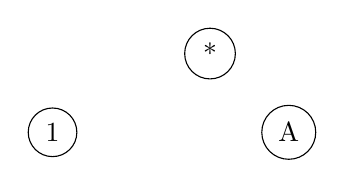
\begin{tikzpicture}
	\node(1) at (0,0) [circle,draw]{1};
		\node(2) at (2,1) [circle,draw]{*};
			\node(3) at (3,0) [circle,draw]{A};
	\end{tikzpicture}
	
	
	
	\subsection{Create Normal Node with various shape:}
	% command for create node: \node(serial_of_node) at(x,y)[name_of_shape,draw]{name_of node}
	\begin{tikzpicture}
		\node(1) at (0,0) [circle,draw]{1};
		\node(2) at (2,1) [draw]{2};
	
	\end{tikzpicture}
	
	
	
	\subsection{Create Normal Node with fill color and face color:}

	% For Fill color: \node(serial_of_node) at(x,y)[circle,color_name,draw]{name_of node}
	%For Face colore:  \node(serial_of_node) at(x,y)[circle,fill=color_name,draw]{name_of node}
	% For face and Fill at time: \node(serial_of_node) at(x,y)[circle,color_name,fill=color_name,draw]{name_of node}
	
	
	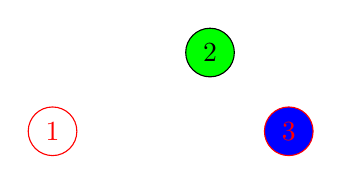
\begin{tikzpicture}
		\node(1) at (0,0) [circle,red,draw]{1};
		\node(2) at (2,1) [circle,fill=green,draw]{2};
		\node(3) at (3,0) [circle,red,fill=blue,draw]{3};
	\end{tikzpicture}
	
	
	
	\subsection{Create a solid node with outside title:}
	%we can use: label=left/right/below/above
	% for size= inner spp= valuept
	%For Text color: text=color_name
	\begin{tikzpicture}
			\node(1) at (0,0)[circle,fill=black,text=white,inner sep=1pt,label=below:A,draw]{};
				\node(1) at (3,0)[circle,fill=black,text=white,inner sep=1pt,label=below:B,draw]{};
	\end{tikzpicture}
	
	
	
	
	
	
	
	\section{Create Edge:}
	\subsection{Normal edge between two node or more node:}
	%--------------------------command for this part-----------------------
	% For create edge: \draw(starting_node) to (ending_node);
	% 2nd Process:     \draw(Starting_node) -- (ending_node);
	%----------------------------------------------------------------------
		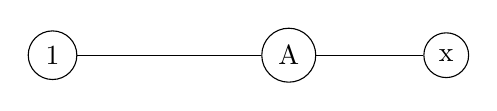
\begin{tikzpicture}
		\node(1) at (0,0) [circle,draw]{1};
		
		\node(2) at (3,0) [circle,draw]{A};
		\node(3) at (5,0)[circle ,draw]{x};
		\draw (1) to (2) to (3);
	\end{tikzpicture}
	
	
	\subsection{Normal edge with arrow between two node or more node:}
	%For create arrow: \draw[->](starting_node) to (ending_node);
	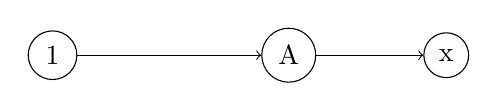
\begin{tikzpicture}
		\node(1) at (0,0) [circle,draw]{1};
		
		\node(2) at (3,0) [circle,draw]{A};
		\node(3) at (5,0)[circle ,draw]{x};
		\draw[->] (1) -- (2);
		\draw[->](2) to (3);
	\end{tikzpicture}
	
	
	
	\subsection{Normal edge with arrow and color between two node or among more node:}
	%For color:\draw[->,color_name](starting_node) to (ending_node);
	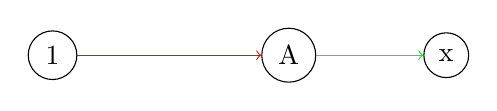
\begin{tikzpicture}
		\node(1) at (0,0) [circle,draw]{1};
		
		\node(2) at (3,0) [circle,draw]{A};
		\node(3) at (5,0)[circle ,draw]{x};
		\draw[->,red] (1) -- (2);
		\draw[->,green](2) to (3);
	\end{tikzpicture}
	
	
	
	
	\subsection{Curve edge with arrow between two node or among more node:}
	%Create: upward curve edge:  \draw[->, bend left=angle] (starting_node) to (ending_node);
	%Create: dawnward curve edge:  \draw[->, bend right=angle] (starting_node) to (ending_node);
	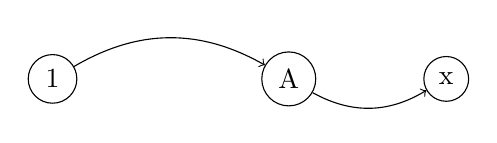
\begin{tikzpicture}
		\node(1) at (0,0) [circle,draw]{1};
		
		\node(2) at (3,0) [circle,draw]{A};
		\node(3) at (5,0)[circle ,draw]{x};
		\draw[->, bend left=30] (1) to (2);
		\draw[->,bend right=30](2) to (3);
	\end{tikzpicture}
	
	
	
	\subsection{Create a self loop in any node:}
	%ctrate: Self loop: \draw[->,loop above](node) to (same_node);
	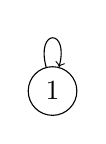
\begin{tikzpicture}
		\node(1) at (0,0) [circle,draw]{1};
	
		\draw[->,loop above](1) to (1);
	\end{tikzpicture}
	\section{Practice section}
	\subsection{practice-1}
	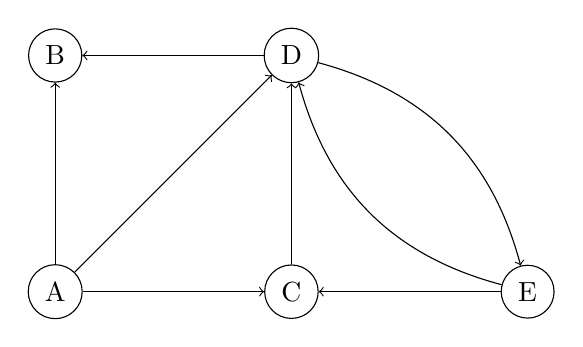
\begin{tikzpicture}
		
		\node(1) at (0,0)[circle,draw]{A};
		\node(2) at (0,3)[circle,draw]{B};
		\node(3) at (3,0)[circle,draw]{C};
		\node(4) at (3,3)[circle,draw]{D};
		\node(5) at (6,0)[circle,draw]{E};
			\draw[->] (1) -- (2);
			\draw[->] (4) -- (2);
			\draw[->] (3) -- (4);
			\draw[->] (1) -- (4);
			\draw[->] (1) -- (3);
			\draw[->] (5) -- (3);
			\draw[->, bend left=30] (4) to (5);
			\draw[->, bend left=30] (5) to (4);
		
	\end{tikzpicture}
	
	
	\subsection{practice-2}
	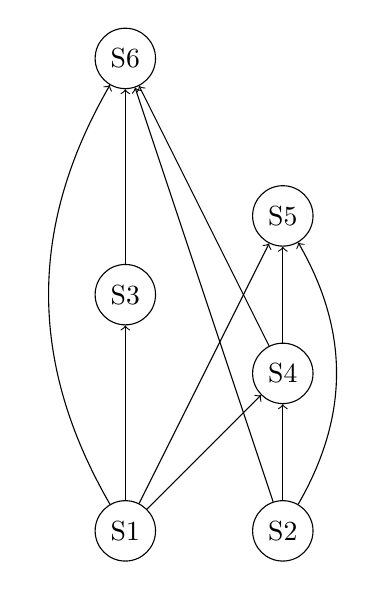
\begin{tikzpicture}
		
		\node(1) at (0,0)[circle,draw]{S3};
		\node(2) at (0,3)[circle,draw]{S6};
		\node(3) at (0,-3)[circle,draw]{S1};
		\node(4) at (2,1)[circle,draw]{S5};
		\node(5) at (2,-1)[circle,draw]{S4};
		\node(6) at (2,-3)[circle,draw]{S2};
		\draw[->] (3) -- (1);
		\draw[->] (1) -- (2);
		\draw[->] (5) -- (2);
		\draw[->] (3) -- (5);
		\draw[->] (6) -- (2);
		\draw[->] (3) -- (4);
		\draw[->] (6) -- (5);
		\draw[->] (5) -- (4);
		\draw[->, bend left=30] (3) to (2);
		\draw[->, bend right=30] (6) to (4);
		
	\end{tikzpicture}
	
	
	
	
		\subsection{practice-3}
	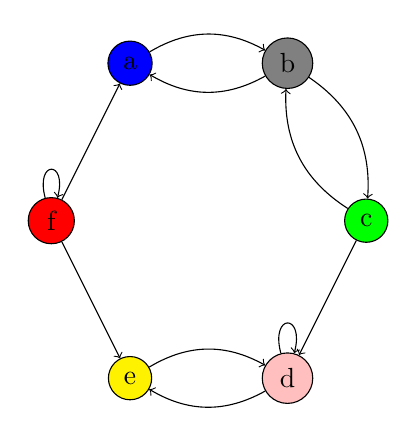
\begin{tikzpicture}
		
		\node(1) at (0,0)[circle,fill=red,draw]{f};
		\node(2) at (4,0)[circle,fill=green,draw]{c};
		\node(3) at (1,-2)[circle,fill=yellow,draw]{e};
		\node(4) at (3,-2)[circle,fill=pink,draw]{d};
		\node(5) at (1,2)[circle,fill= blue,draw]{a};
		\node(6) at (3,2)[circle,fill=gray,draw]{b};
		\draw[->] (1) -- (5);
		\draw[->] (1) -- (3);
		\draw[->] (2) -- (4);
	
		\draw[->, bend left=30] (5) to (6);
		\draw[->, bend left=30] (6) to (5);
		\draw[->, bend left=30] (3) to (4);
		\draw[->, bend left=30] (4) to (3);
		\draw[->, bend left=30] (6) to (2);
		\draw[->, bend left=30] (2) to (6);
		\draw[->,loop above] (1) to (1);
			\draw[->,loop above] (4) to (4);
		
	\end{tikzpicture}
	
	
	\subsection{Practice-4}
	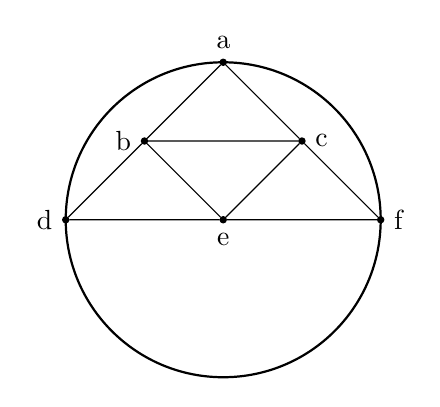
\begin{tikzpicture}
		\node(1) at (0,0)[circle,fill=black,text=white,inner sep=.8pt,label=below:e,draw]{};
		\node(2) at (-2,0)[circle,fill=black,text=white,inner sep=.8pt,label=left:d,draw]{};
		\node(3) at (2,0)[circle,fill=black,text=white,inner sep=.8pt,label=right:f,draw]{};
		\node(4) at (0,2)[circle,fill=black,text=white,inner sep=.8pt,label=above:a,draw]{};
		\node(5) at (-1,1)[circle,fill=black,text=white,inner sep=.8pt,label=left:b,draw]{};
		\node(6) at (1,1)[circle,fill=black,text=white,inner sep=.8pt,label=right:c,draw]{};
		
		\draw (1) to (2) to (5) to (4) to (6) to (3) to (1) to (5) to (6) to (1);
		\draw[thick] (0,0) circle(2);
	\end{tikzpicture}
	
		\subsection{Practice-4}
	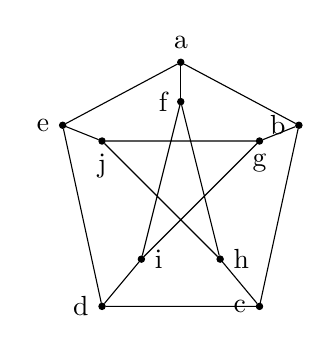
\begin{tikzpicture}
		\node(1) at (-1,1)[circle,fill=black,text=white,inner sep=.8pt,label=below:j,draw]{};
		\node(2) at (1,1)[circle,fill=black,text=white,inner sep=.8pt,label=below:g,draw]{};
		\node(3) at (-.5,-.5)[circle,fill=black,text=white,inner sep=.8pt,label=right:i,draw]{};
		\node(4) at (.5,-.5)[circle,fill=black,text=white,inner sep=.8pt,label=right:h,draw]{};
		\node(5) at (0,1.5)[circle,fill=black,text=white,inner sep=.8pt,label=left:f,draw]{};
		\node(6) at (-1.5,1.2)[circle,fill=black,text=white,inner sep=.8pt,label=left:e,draw]{};
		\node(7) at (0,2)[circle,fill=black,text=white,inner sep=.8pt,label=above:a,draw]{};
		\node(8) at (1.5,1.2)[circle,fill=black,text=white,inner sep=.8pt,label=left:b,draw]{};
		\node(9) at (-1,-1.1)[circle,fill=black,text=white,inner sep=.8pt,label=left:d,draw]{};
		\node(10) at (1,-1.1)[circle,fill=black,text=white,inner sep=.8pt,label=left:c,draw]{};
		
		\draw (1) to (2) to (3) to (5) to (4) to (1) to (6)  to (7) to (8) to (10) to (9) to (3);
		\draw(9) to (6);
		\draw(5) to (7);
		\draw(4) to (10);
		\draw(8) to (2);
		
	\end{tikzpicture}
	
	
	
	
	
	
	
\end{document}